\section{Model System for the Precision Agriculture System}

\begin{figure}[H]

	\centering

 	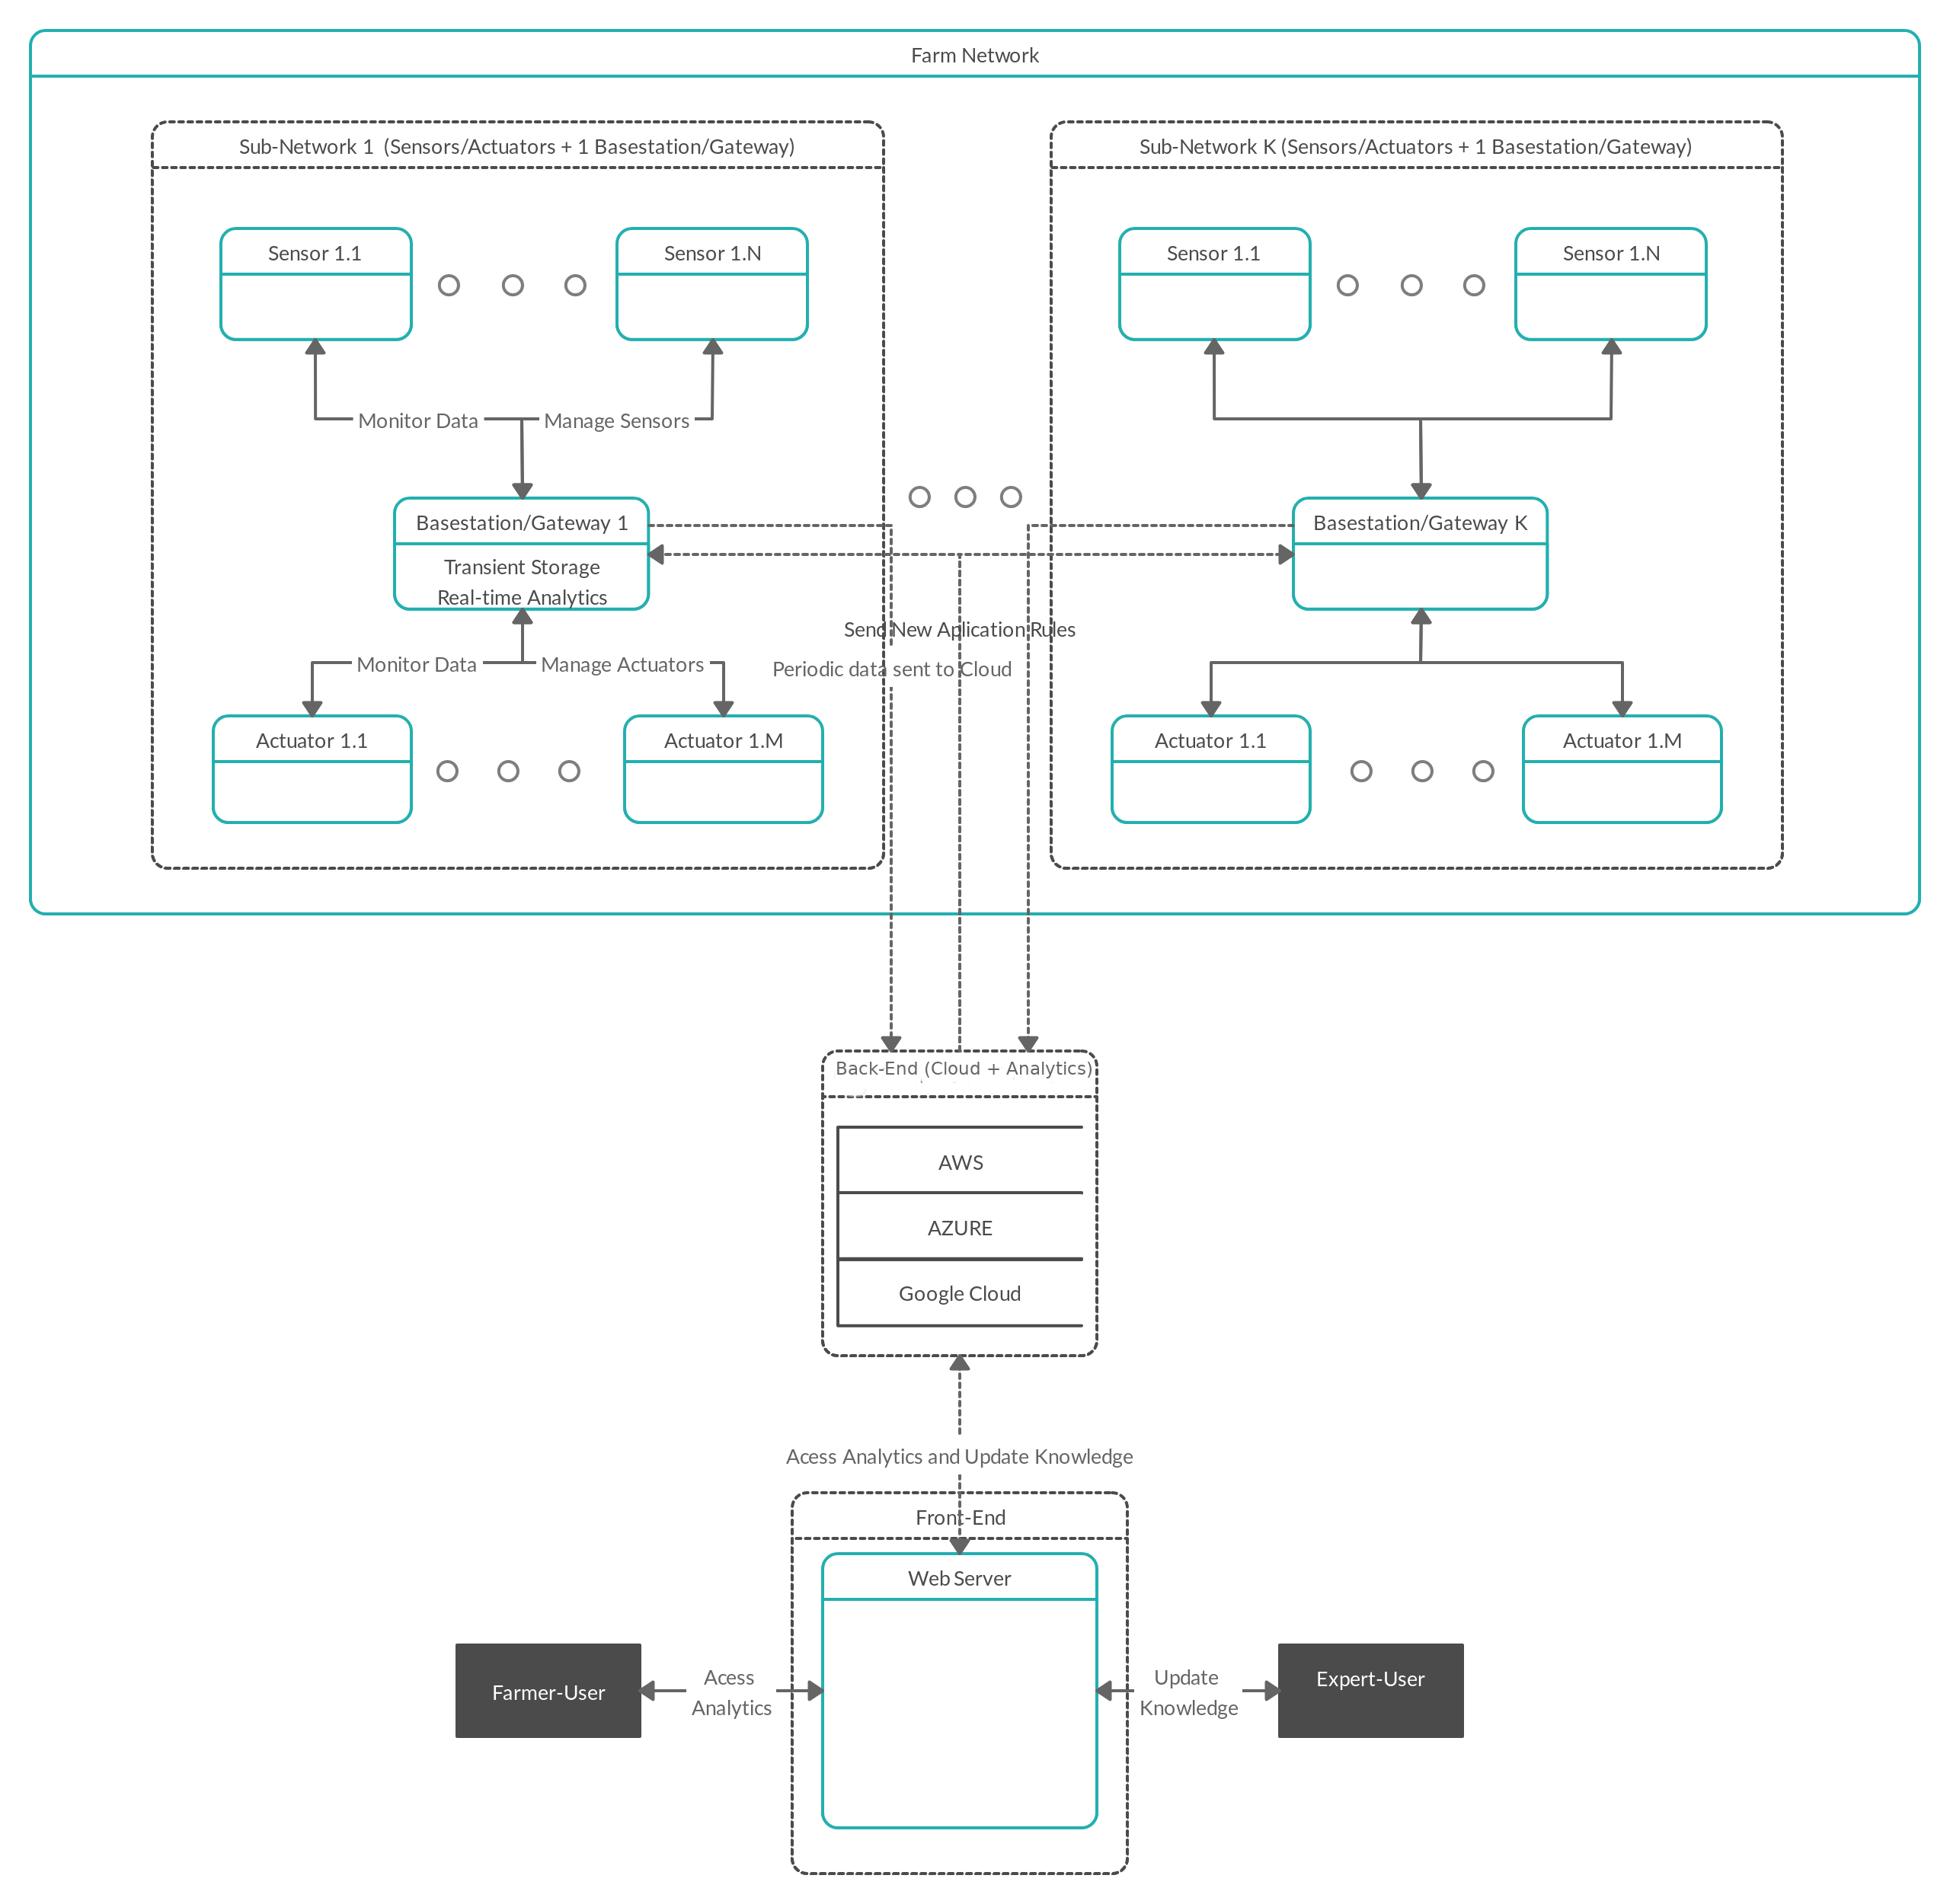
\includegraphics[scale = 0.15]{precisionAgricultureSystem.png}

 	\caption {Model System for the Precision Agriculture System}

  	\label{fig01}
\end{figure}

	O sistema encontra-se dividido em três boundaries principais a cloud, o sistema de agricultura e o front-end. Ainda dentro da boundary do sistema de agricultura divide-se em pequenos sub-sistemas que correspondem ao conjunto de uma basestation/gateway junto com os sensores e actuators.

	A partir do modelo entende-se que os sub-sistemas referidos anteriormente não comunicam entre si, só com a cloud , de forma a atualizar as configurações das basestations/Gateways e a transmitir a informação recolhida pelos sensores á front-end. Também o back-end, formado pelo armazenamento em cloud e o modulo de analytics, só deve comunicar com as basestations/gateways e com o servidor do front-end fornecendo uma API para comunicar com o mesmo. Finalmente, temos o front-end que para além da Cloud só comunica com dois tipos de utilizadores externos ao sistema que são os agricultores e os Experts.

	É importante salientar que o back-end deste sistema é responsabilidade dos fornecedores de serviços indicados na figura, o que, por si só, já fornece algumas garantias de segurança para o próprio sistema de armazenamento. Na seção seguinte analisar-se-á mais detalhadamente cada parte deste sistema de forma a encontrar possíveis ameaças subjacentes a essas boundaries e elementos.

	Nas duas seguintes imagens encontram-se generalizados os processos executados pelos dois tipos de utilizadores do nosso sistema. Apesar de se encontrar representado o acesso aos dados pelo Farmer, é esperado que o Expert também os requisite. No entanto, só o Expert é que poderá alterar os dados da base dados para melhorar o funcionamento do sistema.

\begin{figure}[h!]

	\centering

 	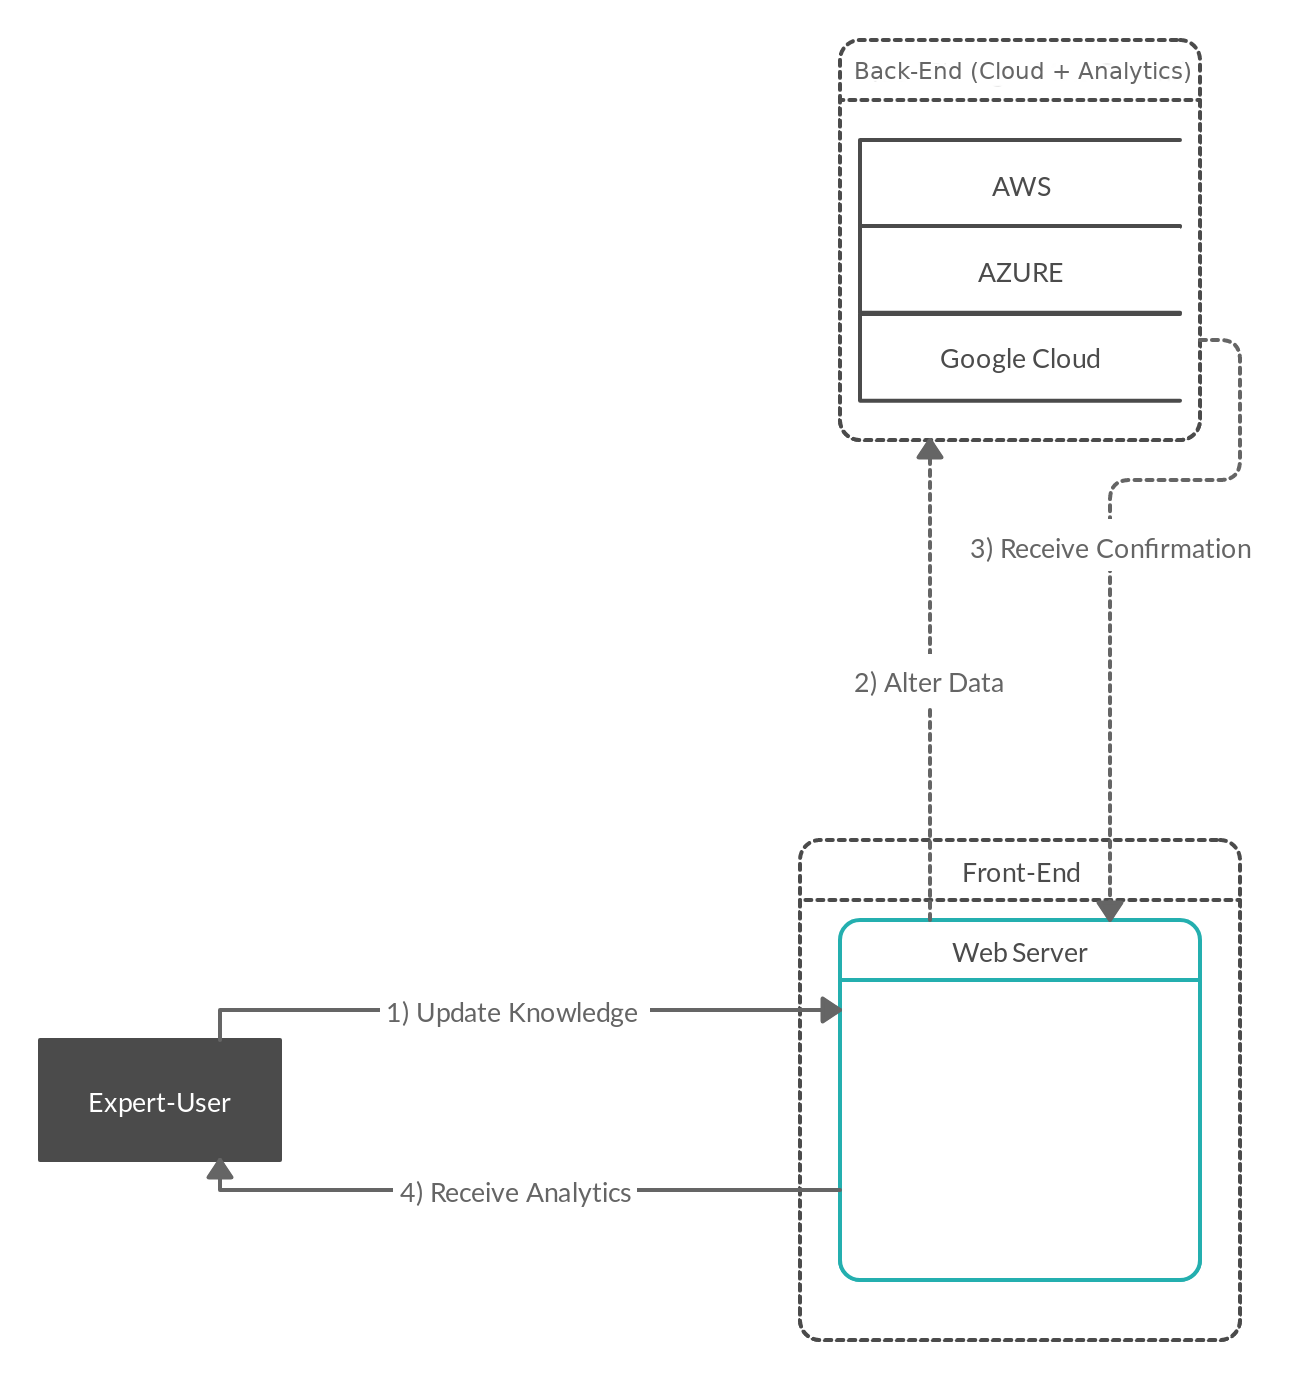
\includegraphics[scale = 0.15]{ExpertAlter.png}

 	\caption {Uploading Data by Expert}

  	\label{fig02}
\end{figure}



\begin{figure}[h!]

	\centering

 	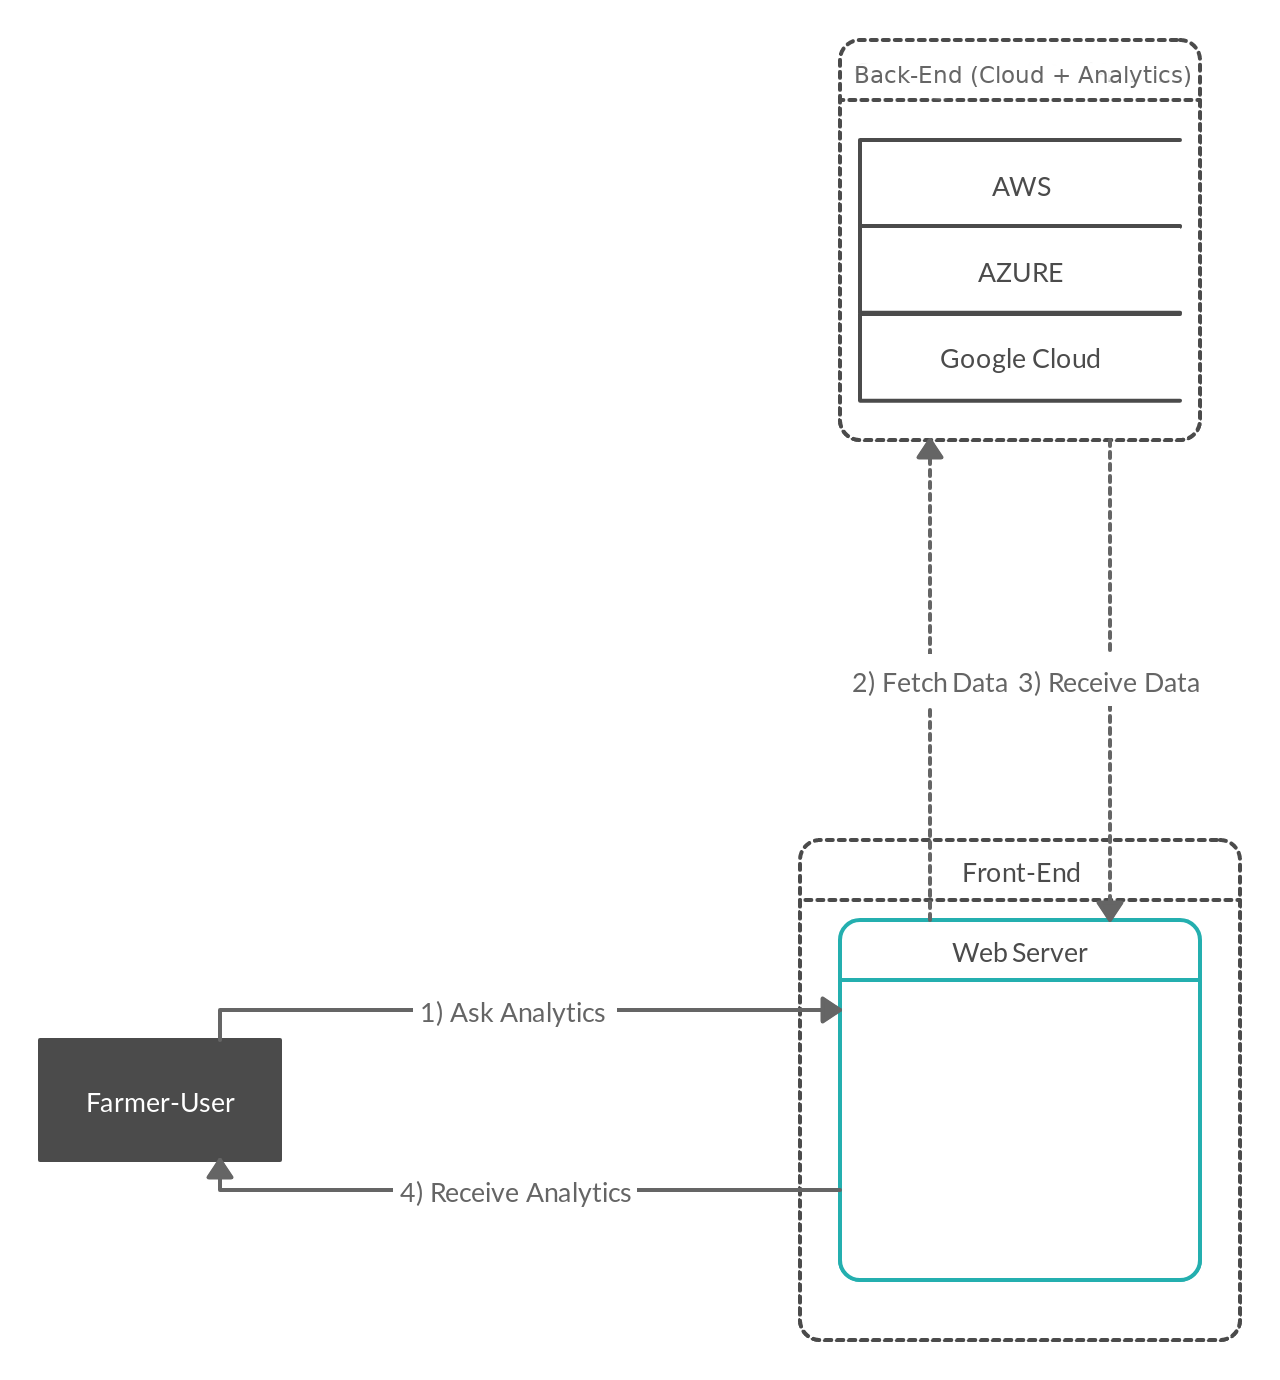
\includegraphics[scale = 0.15]{FarmerAcess.png}

 	\caption {Acessing Data by Farmer}

  	\label{fig03}
\end{figure}

No subsistema da quinta identificam-se 3 processos nos quais o \"data flow\" pode sofrer ataques devido a vulnerabilidades. Na figura 4 podemos ver os "actuators" que controlam a temperatura/humidade das zonas da quinta. As basestations que coletam a informação recolhida pelos sensores e a Cloud para a qual enviam a informação recolhida e da qual recebem instruções.

\begin{figure}[H]

	\centering

 	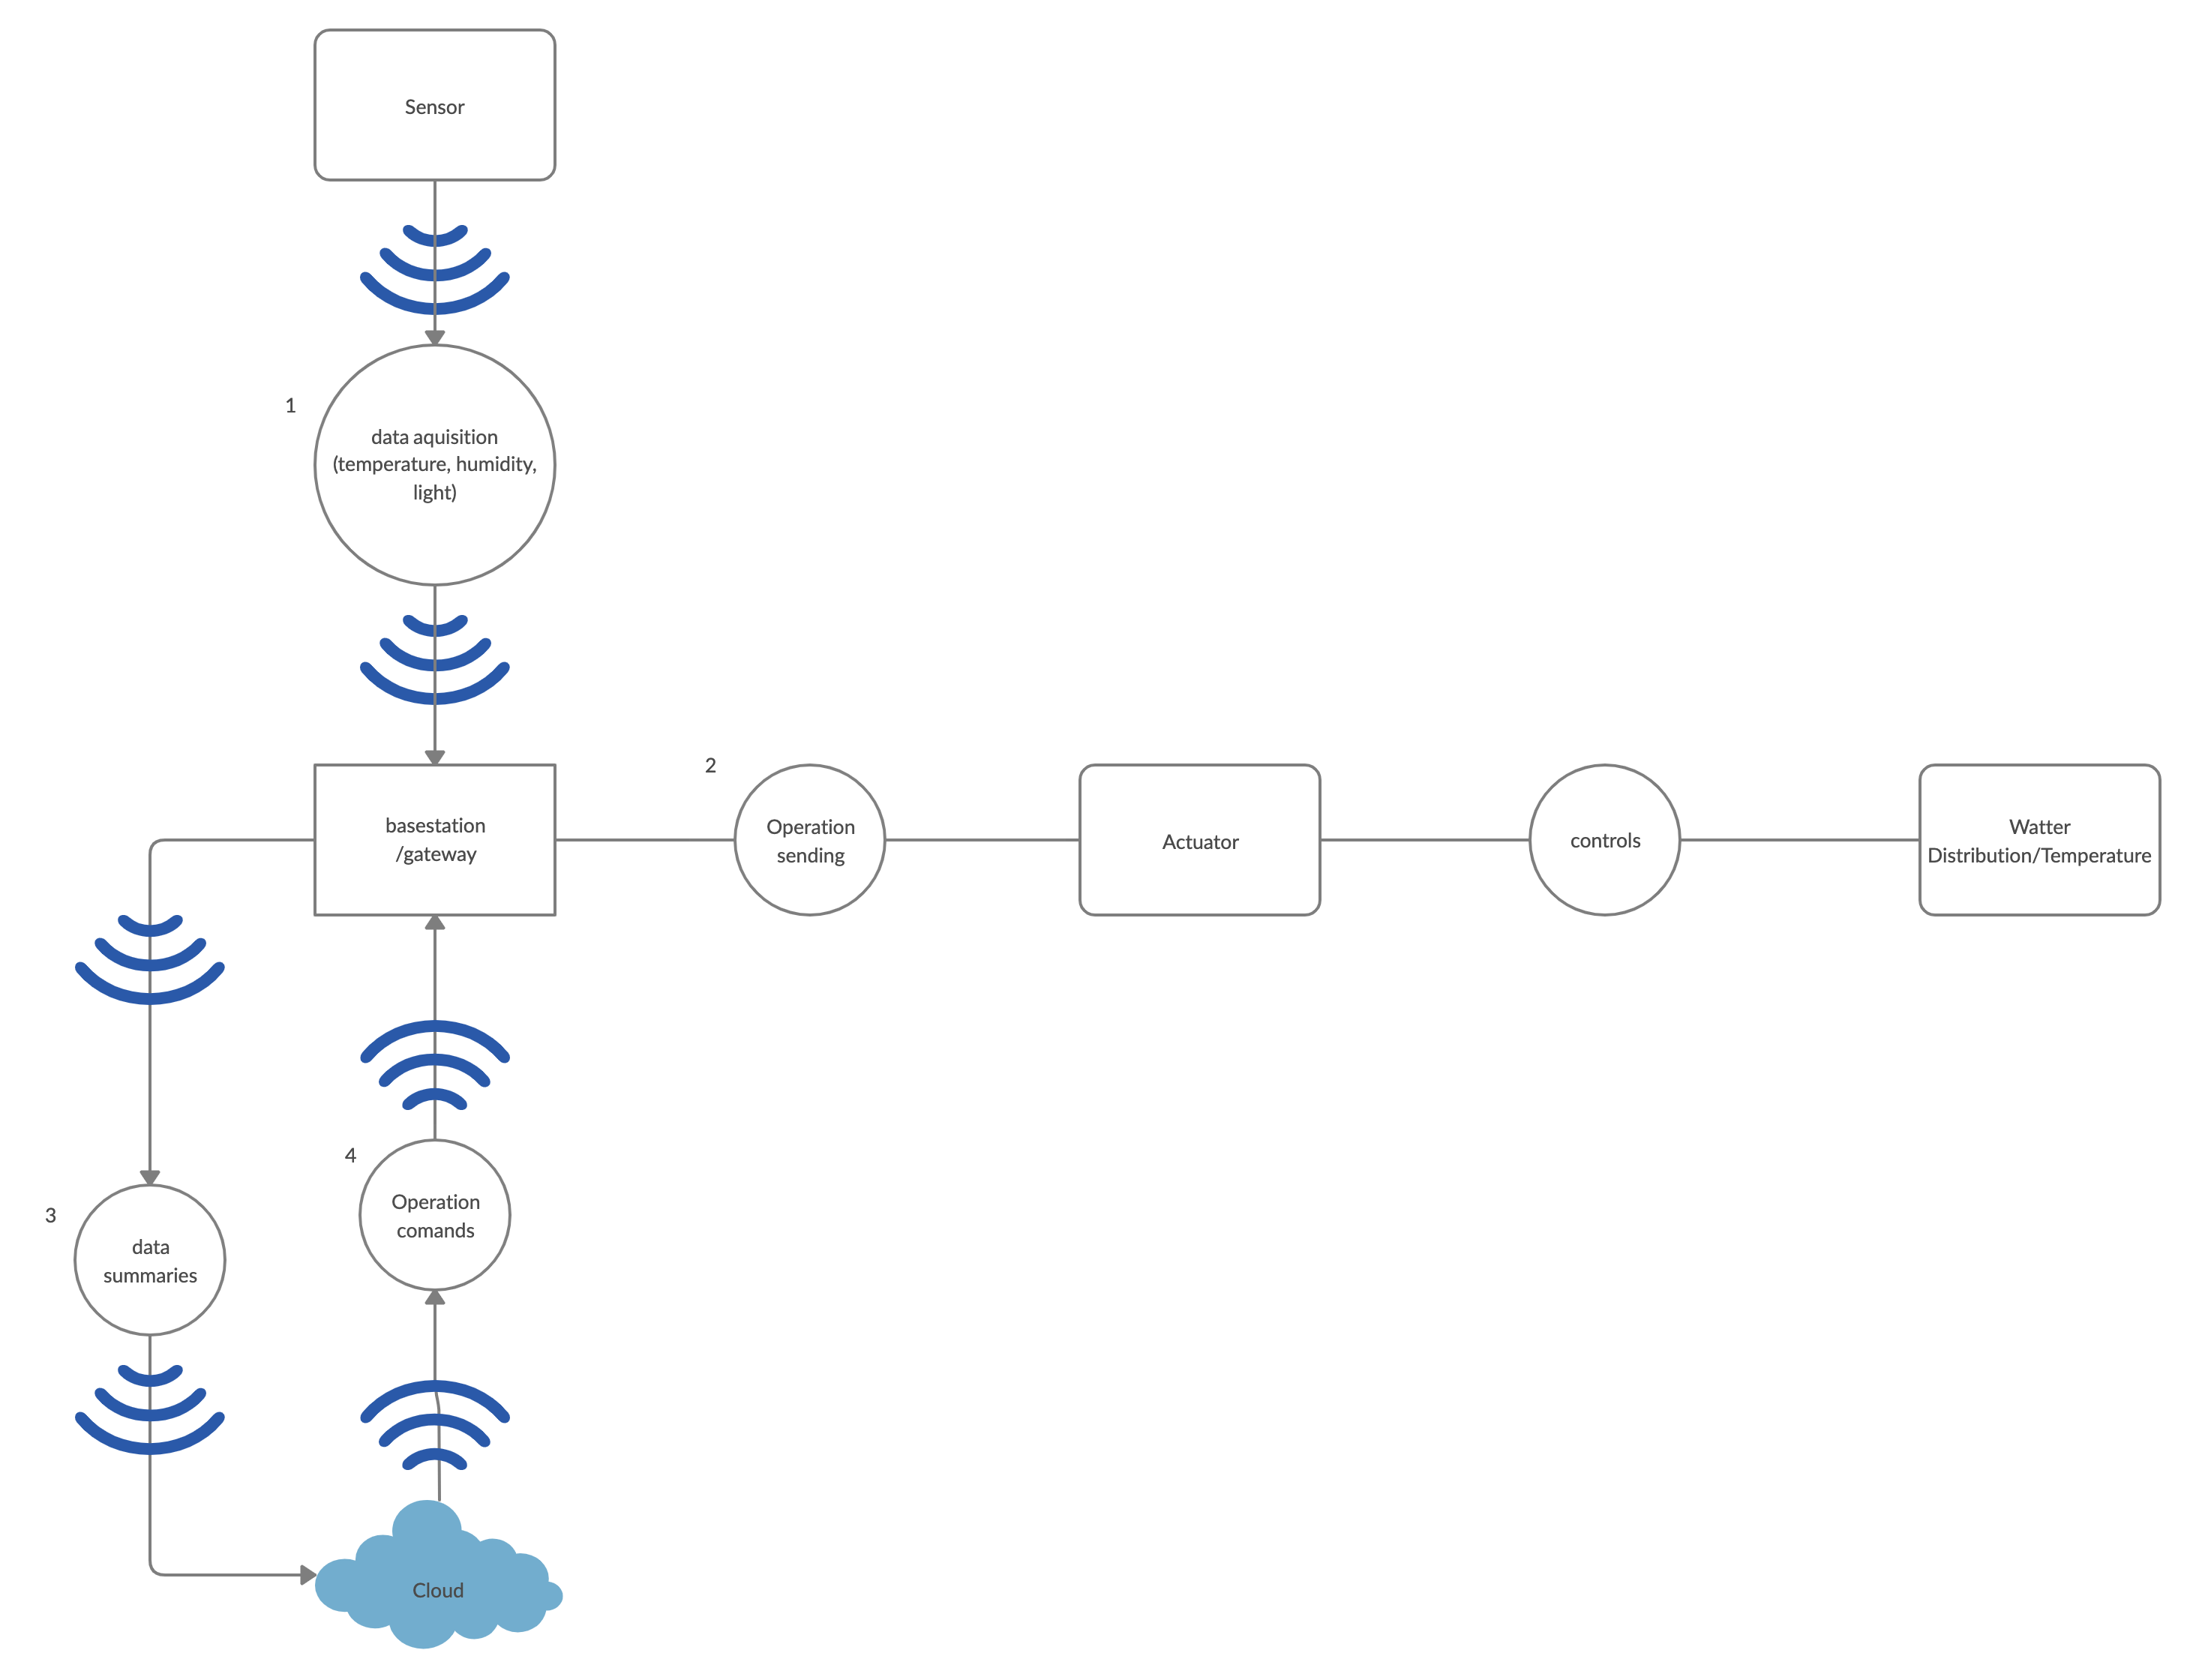
\includegraphics[scale = 0.1]{farmModel.png}

 	\caption {Model System for the Farm Subsystem}

  	\label {fig04}
\end{figure}

\section{Finding \& Addressing Threats}

	De forma a encontrar as ameaças referentes ao sistema ir-se-á analisar cada elemento seguindo STRIDE.Cada subseção corresponde a um dos três subsistemas definidos anteriormente.



\subsection{FrontEnd}

\subsubsection{Spoofing}
\label{Spoofing:sec}
\hfill\\
\begin{itemize}

\item Um atacante poderia conetar ao sistema em 1) e 3) em  na figura \ref{fig02} ou em \ref{fig03} caso este nao tenha nenhum sistema de autentificação tanto para os utilizadores do Front-end como para o Front-end em si ao conetar-se ao Back-End. Para mitigar esta ameaça é necessário tanto um sistema de autentificação para os utilizadores (login) como um sistema para gerenciar as sessões do mesmo(Encrypted cookies,Session Keys). Enquanto na ligação do Front-End ao Back-End é também necessário alguma forma de Autentificação(Tickets Kerberos,IPsec). Assim, só se permitiria aos servidores Front-End autorizados aceder a API do Back-End e solicitar dados do mesmo.

\hfill\\
\item Um atacante em 1) poderia tentar fazer login na aplicaçao front-end como farmer/Expert através de tentativas sucessivas de pares user/password. De forma a mitigar o problema poder-se-ia implementar um  delay quando o sistema nota muitas tentativas de login. Esta medida tem consequências visto que pode ser prejudicial ao sistema.
 Mesmo que o atacante não conseguisse descobrir os pares login/password, caso este processo de tentativa de adivinhação fosse realizado inumeras vezes num curto espaço de tempo, o mesmo ataque passaria a um DoS impedindo que os utilizadores do Front-End se conseguissem conectar ao sistema. Possivelmente uma Firewall ajudaria a mitigar esta ameaça.


\hfill\\
\item Um atacante poderia criar um "clone" do web-server de forma a enganar o cliente para inserir os dados de login. Assim obtendo acesso ao sistema ao nivel do utilizador. A mitigação deste ataque é possível através do uso de credenciais no Front-End que serão guardadas pelo browser do utilizador. 

\hfill\\
\item Um atacante irá sempre utilizar o método com a segurança mais fraca. Consequentemente, dever-se-á obrigar sempre a utilização das ligações com protocolos que possuam encriptaçao(HTTPS/IPsec).

\end{itemize}

\subsubsection{Tampering}
\hfill\\
\begin{itemize}

\item Um atacante poderia alterar dados referentes ao sensores no web server na figura \ref{fig02}, de forma a enganar o cliente sobre o estado dos sensores e da quinta. Utilizando um mecanismo de encriptação nos dados este ataque pode ser mitigado.

\end{itemize}

\subsubsection{Repudiation}
\hfill\\
\begin{itemize}

\item Um utilizador do tipo Expert poderia em 1) na figura \ref{fig03} mandar um pedido para alterar a knowledge do sistema de forma a piorá-lo e não admitir essa alteraçao. Para evitar esta situação poderia manter Logs de alterações feito pelos Experts no armazenamento na Cloud.

\end{itemize}

\subsubsection{Information Disclosure}
\hfill\\
\begin{itemize}
\item Admitindo que a aplicação pode dar suporte a diferentes farms. Um utilizador ja ligado ao sistema pertencente á concorrência poderia pedir acesso a ficheiros dos concorrentes. Uma solução fácil seria implementar ACLs para restringir acesso aos ficheiros ou na lógica da aplicação WEB do Front-End.

\hfill\\

\item Outros problemas como man-in-middle, acesso ao ficheiro não encriptado,etc. Sao resolvidos com alguns do métodos referidos anteriormente.
\end{itemize}

\subsubsection{Denial of Service}
\hfill\\
\begin{itemize}

\item Como referido na seção de Spoofing no primeiro ponto, poderia causar-se DoS usando o delay para prevenir tentativas de brute force das passwords.

\hfill\\
\item Um atacante depois de entrar no sistema Front-End como Expert pode tentar atualizar o sistema através de vários PCs com login na mesma conta. Provocando uma incapacidade do Servidor para que este não conseguisse satisfazer todos os pedidos. O mesmo poderia ser feito caso fosse feito login como Farmer através de varios GETs. O Profiling do tráfego da rede como anomalias e reputações de IP mitigariam o ataque.

\end{itemize}

\subsubsection{Elevation of Privilege}
\hfill\\

\begin{itemize}

\item Um atacante não ligado ao sistema pode tentar utilizar a API para aceder ao Back-End.Ganhando assim os mesmos privilegios que o servidor Front-End.Uma lista com os servidores/utilizadores que podem aceder diretamente a API podia mitigar este ataque.

\end{itemize}

\hfill\\


